\chapter{Implementation - "Building the solution"}


\section{Introduction}

This chapter is a walkthrough of the steps which describe the construction of the application.

\section{Initial Setup}

\subsection{Command Line Instructions}

As this application was centred towards security and being secure as the data it would hold would need to be kept safe. Therefore it made sense to focus on a good login with authentication and authorisation. To start working with Symfony, one needs to setup the Symfony enviroment through an installation process before Symfony applications can be created. Instructions for this can be found on the SensioLabs Symfony website. Navigating to the Documentation page. In there can be found Chapter 1 which has the Setup instructions under the Get Started dropdown menu. They explain the different ways for installing and setting up the Symfony framework for both Mac OS and Windows. Along with some\newline troubleshooting ideas if there are any problems with the installation. This application was built on a Mac OS so the instructions would vary slightly due to the command line instructions used. Using the installer made it easy to create this application with Symfony and only needed to be done once as it was installed globally on the machine.

\begin{figure}[htbp]
   \centering
   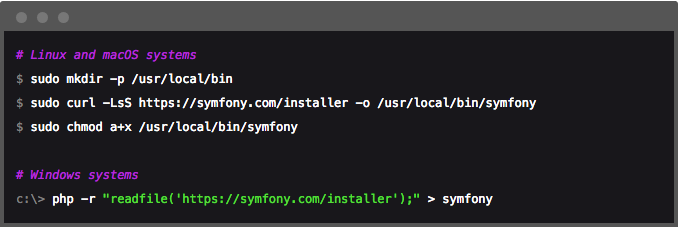
\includegraphics[width=400pt]{figures/symfony_installation.png} % requires the graphicx package
   \caption{Symfony Installation Setup}
   \label{fig:Symfony Installation Setup}
\end{figure}

With this completed moving into the directory where the application would be deployed from. A final command in the terminal window was issued. This time starting with symfony new and by giving a project a name of choice thereafter. In this case the name\newline COMPH4021-Project was used. The project was based on the current version of Symfony which is version 3.2. However, other versions can be specified after the project name in the terminal window. Once this part was completed. All required components were downloaded into a project folder with the name of which was given. The components are a set of files and directories which form the web application which use the Symfony libraries. The installer also carries out a check to make sure all requirements are met. If requirements are not all met a list is generated which provides the changes that are needed. In this case no changes needed to be made.

\begin{figure}[htbp]
   \centering
   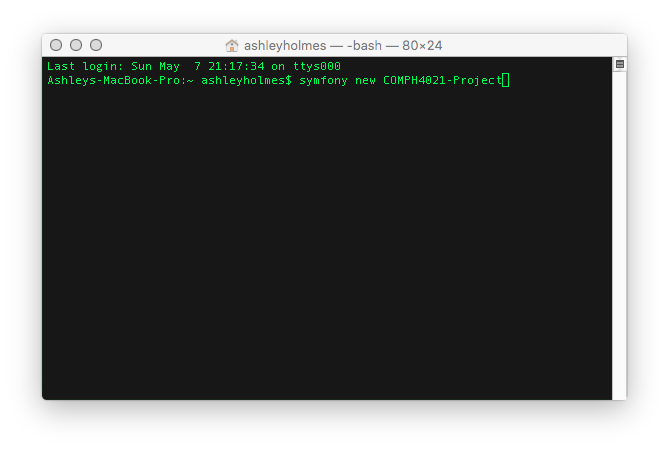
\includegraphics[width=400pt]{figures/new_application.png} % requires the graphicx package
   \caption{Symfony Application Setup}
   \label{fig:Symfony Application Setup}
\end{figure}

The below figure \ref{fig:Terminal Window Top} displays the command issued to download the project folder and following that in figure \ref{fig:Terminal Window Bottom} one can see that the project is being prepared and where it will be stored. In this case it was stored in /Users/ashleyholmes/Desktop/COMPH4021-Project.

\begin{figure}[htbp]
   \centering
   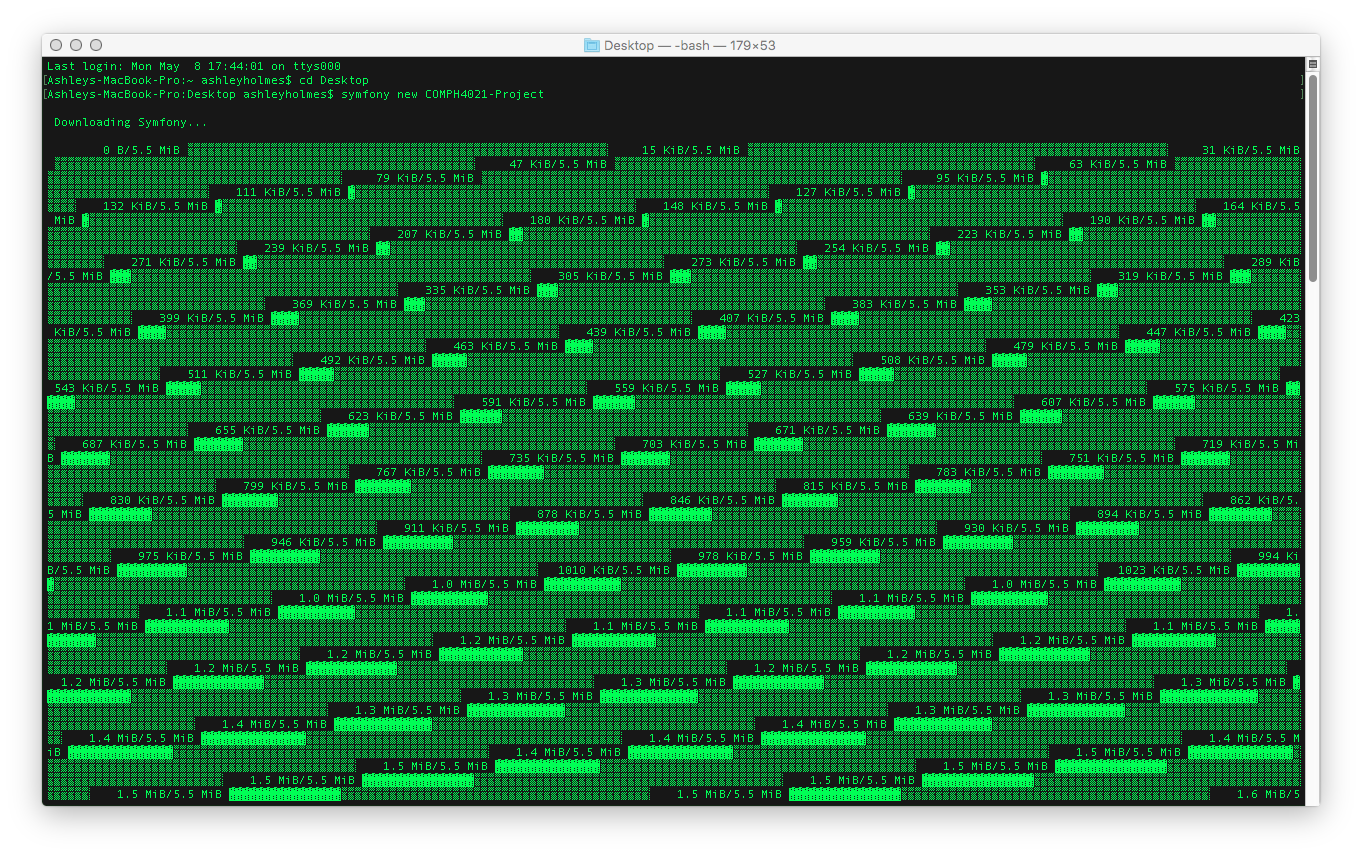
\includegraphics[width=400pt]{figures/terminal_window_top.png} % requires the graphicx package
   \caption{Terminal Window Top}
   \label{fig:Terminal Window Top}
\end{figure}

\begin{figure}[htbp]
   \centering
   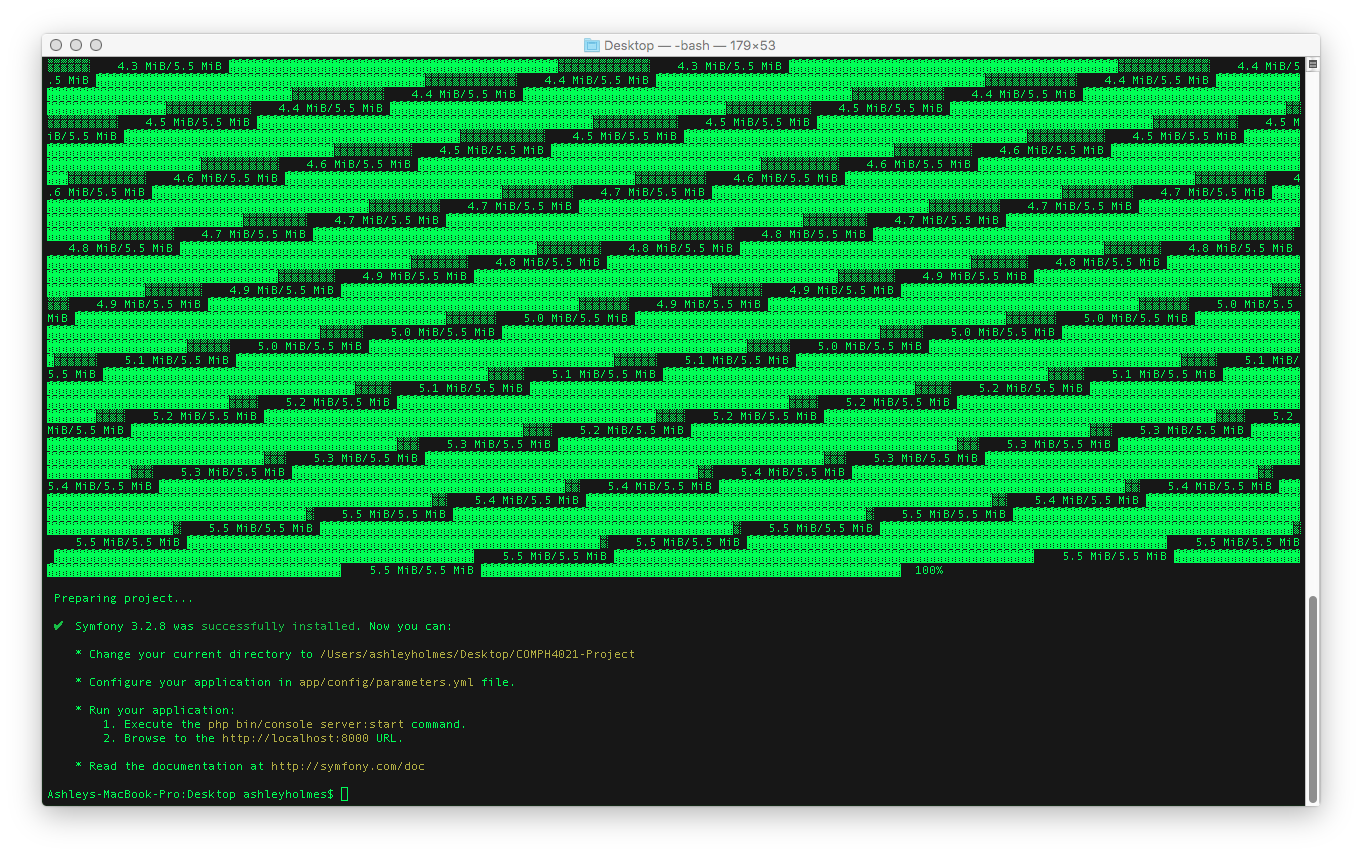
\includegraphics[width=400pt]{figures/terminal_window_bottom.png} % requires the graphicx package
   \caption{Terminal Window Bottom}
   \label{fig:Terminal Window Bottom}
\end{figure}

The next step would be to change directory into the COMPH4021-Project directory as this is where the built in PHP server needs to be run from. Engine Executing the following command php bin/console server:run starts the server. However, once issuing this command the open terminal window would now need to remain out of use while the server is running. One can use a separate terminal window or open a new tab to issue any addition commands which are needed or make use of the PhpStorm terminal window. To avoid doing all of this issuing a php bin/console server:start will make it possible to execute commands in the same window which was done here. The difference can be seen in figure \ref{fig:Php Server Run} and figure \ref{fig:Php Server Start}.

\begin{figure}[htbp]
   \centering
   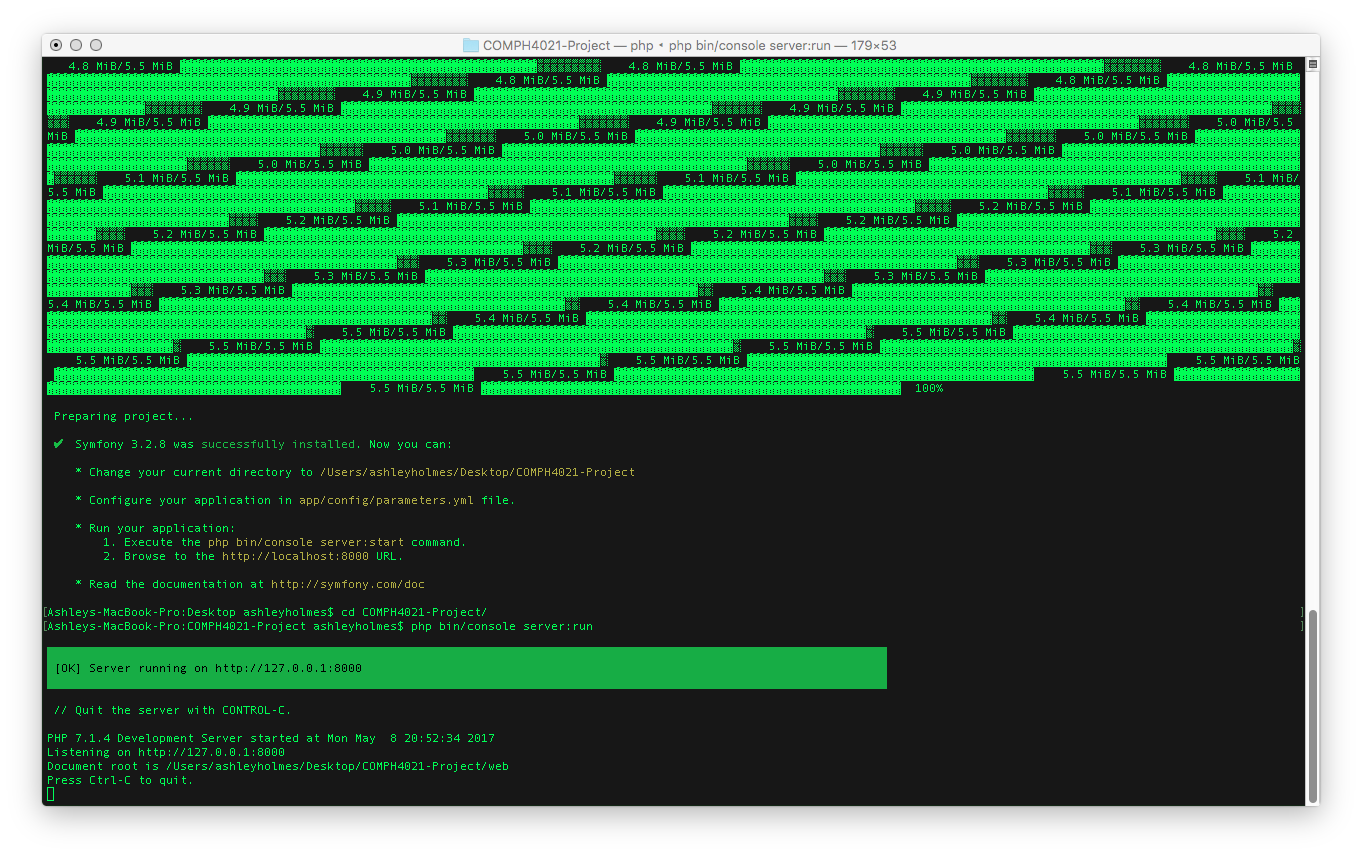
\includegraphics[width=400pt]{figures/php_server_run.png} % requires the graphicx package
   \caption{Php Server Run}
   \label{fig:Php Server Run}
\end{figure}

\begin{figure}[htbp]
   \centering
   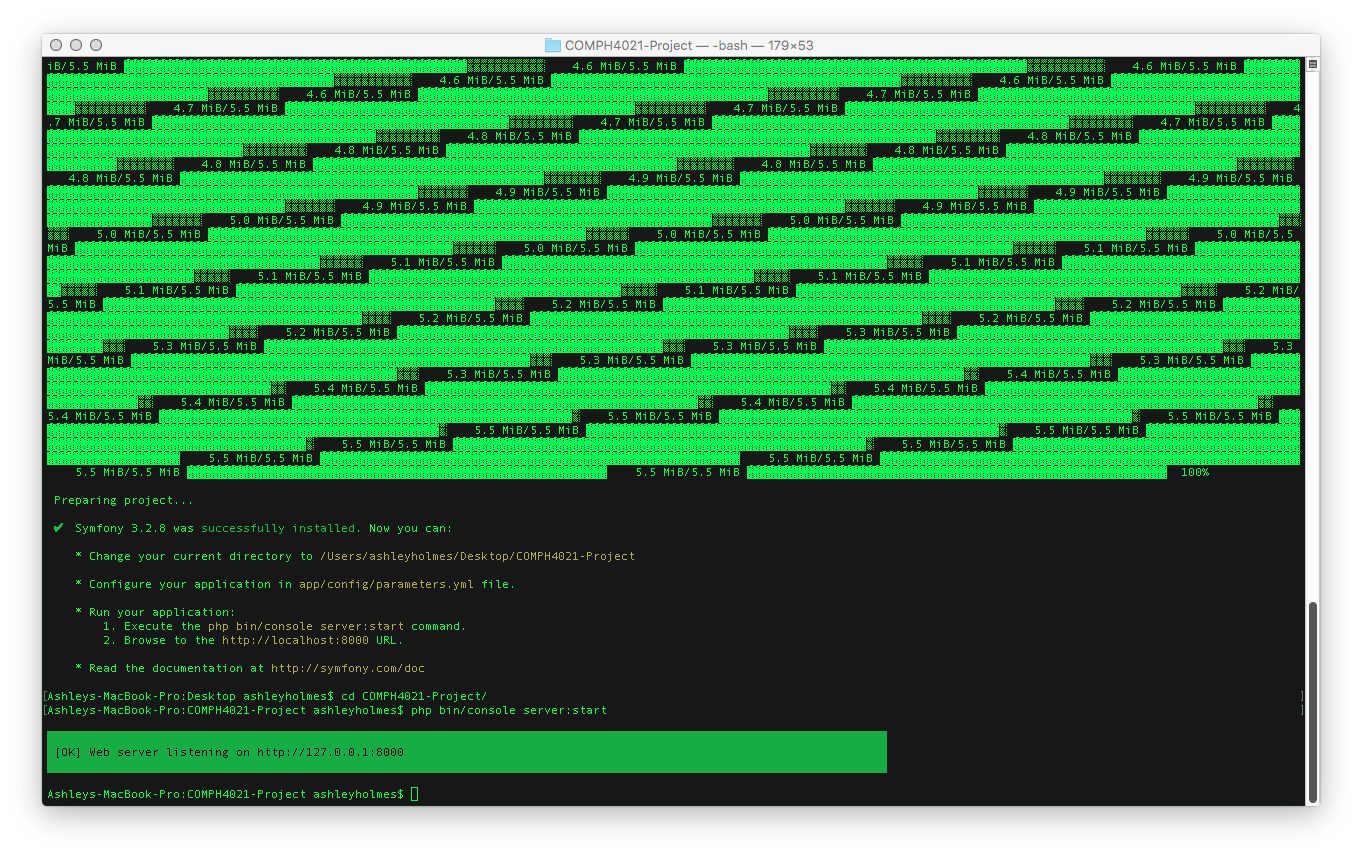
\includegraphics[width=400pt]{figures/php_server_start.png} % requires the graphicx package
   \caption{Php Server Start}
   \label{fig:Php Server Start}
\end{figure}

\section{Browser}

\subsection{Deploying the Application}

Now that the configuration phase has been complete